\begin{question}[section=11,name={Helmholtz},difficulty=,quantity=,type=thr,tags={}]
	Wie lautet die Lösung der inhomogenen Helmholtzgleichung für das Vektorpotential $\vec{A}$ bei bekannter Dichte der eingeprägten Ströme $\vec{S_e}$? Zeichnen sie eine Skizze der Geometrie!
	\\ \textbf{Hinweis:}\\
	
\end{question}
\begin{solution}
	$\vec{A}(\vec{r}) = \frac{\mu}{4 \pi} \cdot \int{\frac{\vec{S_e}(\vec{r})\cdot e^{-jk|\vec{r}- \vec{r'}|}}{|\vec{r}- \vec{r'}|} \partial V'}$ \\
	\begin{figure}[H]
		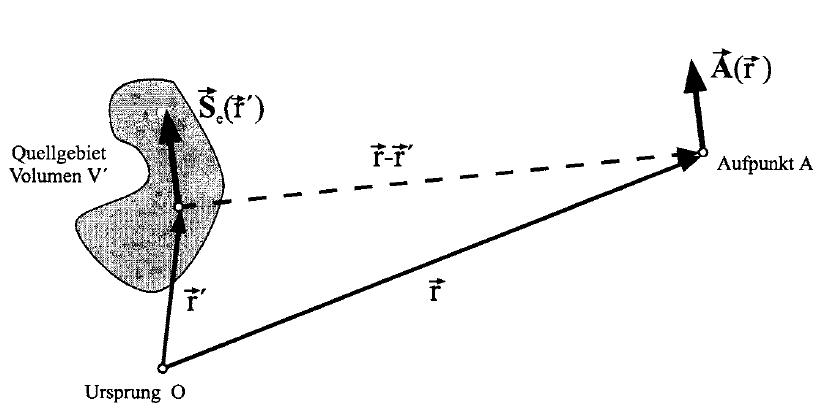
\includegraphics[width=14cm]{./opn/exm/thr/chp/11/5/bild.jpeg}
	\end{figure}
\end{solution}